\documentclass{beamer}
%\usetheme{Antibes}
\usetheme{Darmstadt}
\usepackage[noae]{Sweave}
%\usepackage{multirow}
%\usepackage{verbatim} 
\newcommand{\R}[1]{\texttt{#1}}
\usepackage{graphicx}
\DeclareGraphicsExtensions{.pdf,.png,.jpg}

\title{Exploratory Data Analysis}
\author{Damian Thomas}
\date{2017-02-03}

\begin{document}

%===============================================================================


%---------------------------------------
\begin{frame}
\maketitle
\end{frame}



%---------------------------------------
\begin{frame}
\frametitle{Topics}
\tableofcontents
\end{frame}



%---------------------------------------
\section{Exploratory Data Analysis}
\subsection{What is it?} 
\begin{frame}
\frametitle{What is Exploratory Data Analysis?} 

\begin{quote}
In statistics, exploratory data analysis (EDA) is an approach to analyzing data sets to summarize their main characteristics, often with visual methods.\footnote{Source: \url{https://en.Wikipedia.org/wiki/Exploratory_data_analysis}}
\end{quote}

\end{frame}


%---------------------------------------
\subsection{History}
\begin{frame}
\frametitle{History} 

The history of R is directly tied to EDA
\begin{itemize}
\item John Tukey works for Bell Labs
\item John Tukey writes a book: Exploratory Data Analysis, Tukey, (1977).
\item Bell Labs develops the S language
\item S-Plus is commerically successful
\item R created -- an open source implementation of the S language
\end{itemize}


\end{frame}



%---------------------------------------
\begin{frame}
\frametitle{EDA is:}

\begin{itemize}
\item Data focused
\item Informal. No model is specified
\item Gain insight into the data generating process. 
\item Learn about the data, underlying structure
\item Summarize the data without losing information. 
\item Gather key information required to build a model. 
\item Generate questions 
\item help decide what sort of model fits
\end{itemize}

\end{frame}



%---------------------------------------
\begin{frame}
\frametitle{EDA is \em{not}:}

\begin{itemize}
\item Model focused
\item Dependent on assumptions (randomness, normality, etc.)
\item A rigorous formal approach
\item Model Specification (regressions, ANOVA)
\item Parameter estimation
\item Hypothesis testing \slash statistical inference
\end{itemize}

\end{frame}



%---------------------------------------
\subsection{Techniques}
\begin{frame}

\frametitle{Techniques}
\begin{itemize}
\item Tukey's five number summary (for any distribution)
    \begin{itemize}
    \item minimum: smallest value
    \item lower quartile: 25th percentile
    \item median: middle value
    \item upper quartile: 75th percentile
    \item maximum: largest value
    \end{itemize}
\item Summary statistics: characterize the distribution
    \begin{itemize}
    \item Extremes: range (minimum and maximum)
    \item Location: median, mean
    \item Spread: quartiles, standard deviation
    \item Shape: modality, skew
    \end{itemize}
\item Visualizations: Present the data, facilitate discovery
    \begin{itemize}
    \item Box plot
    \item Scatter plot
    \item Line plot
    \item Bar plot
    \item Histogram
    \end{itemize}
\end{itemize}

\end{frame}


%---------------------------------------
\section{Data Analysis Process}
\begin{frame}
\frametitle{The Data Analysis Process\footnote{Source: R for Data Science \url{http://r4ds.had.co.nz/}}}


\begin{figure}
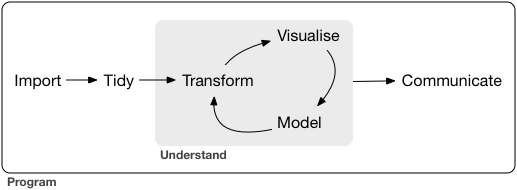
\includegraphics[width=0.8\textwidth,natwidth=610,natheight=642]{images/data-science}
\end{figure}

\begin{itemize}
\item Write code to carry out each step
\item Save the code so you can reproduce (and share) your work
\end{itemize}

\end{frame}


%---------------------------------------
\subsection{Import}
\begin{frame}
\frametitle{Get raw data}
Start by getting the data
\end{frame}



%---------------------------------------
\subsection{Tidy}
\begin{frame}
\frametitle{Tidy Data}
Apply tidy principles and restructure your data if necessary

\begin{itemize}
\item Each variable should have its own column
\item Each observation should have its own row
\item Each value  should have its own cell
\end{itemize}

\end{frame}



%---------------------------------------
\subsection{Transform}
\begin{frame}
\frametitle{Transform}

Create new variables, change existing ones, remove extraneous information.
\end{frame}



%---------------------------------------
\subsection{Model}
\begin{frame}
\frametitle{Model}

Use what you've learned to specify a model and apply classical statistics to confirm exporatory findings

\end{frame}



%---------------------------------------
\subsection{Iterate}
\begin{frame}
\frametitle{Iterate}
Continue to refine the analysis. Use what you learn to ask more questions and learn more about the data.
\end{frame}



%---------------------------------------
\subsection{Communicate}
\begin{frame}
\frametitle{Communicate}
Share your results
\end{frame}



%---------------------------------------
\section{Example: Anscombe's Quartet}
\begin{frame}[fragile]
\frametitle{Example Data Sets: Anscombe's Quartet}

\begin{quote}
Anscombe's quartet comprises four datasets that have nearly identical simple descriptive statistics, yet appear very different when graphed. Each dataset consists of eleven (x,y) points. They were constructed in 1973 by the statistician Francis Anscombe to demonstrate both the importance of graphing data before analyzing it and the effect of outliers on statistical properties.\footnote{Source: \url{http://en.wikipedia.org/wiki/Anscombe's_quartet}}
\end{quote}

\end{frame}



%---------------------------------------
\subsection{Import Data}
\begin{frame}[fragile]
\frametitle{read.table() family of functions}

\begin{Schunk}
\begin{Sinput}
> ?read.table()
> ?read.csv()
> ?read.delim()
\end{Sinput}
\end{Schunk}

These functions read raw data saved in delimitied text files, and return a data frame object.

\end{frame}


%---------------------------------------
\begin{frame}[fragile]
\frametitle{Read raw data from a csv file}

\begin{Schunk}
\begin{Sinput}
> anscombe <- read.csv("data/anscombe.csv", 
+                      stringsAsFactors = FALSE)
\end{Sinput}
\end{Schunk}
\pause
\begin{Schunk}
\begin{Sinput}
> anscombe
\end{Sinput}
\begin{Soutput}
   x1 x2 x3 x4    y1   y2    y3    y4
1  10 10 10  8  8.04 9.14  7.46  6.58
2   8  8  8  8  6.95 8.14  6.77  5.76
3  13 13 13  8  7.58 8.74 12.74  7.71
4   9  9  9  8  8.81 8.77  7.11  8.84
5  11 11 11  8  8.33 9.26  7.81  8.47
6  14 14 14  8  9.96 8.10  8.84  7.04
7   6  6  6  8  7.24 6.13  6.08  5.25
8   4  4  4 19  4.26 3.10  5.39 12.50
9  12 12 12  8 10.84 9.13  8.15  5.56
10  7  7  7  8  4.82 7.26  6.42  7.91
11  5  5  5  8  5.68 4.74  5.73  6.89
\end{Soutput}
\end{Schunk}

\end{frame}



%---------------------------------------
\subsection{Tidy Data}
\begin{frame}[fragile]
\frametitle{Tidy Data Checklist}

\begin{itemize}
\item<1-1> Each value should have its own cell.
\item<2-> PASS: Each value  should have its own cell. \par Every cell has a single value.
\item<3-3> Each variable should have its own column.
\item<4-> PASS: Each variable should have its own column. \par Every column is uniquely named and has one kind of data.
\item<5-5> Each observation should have its own row.
\item<6-> FAIL: Each observation should have its own row. \par Anscombe's quartet is comprised four separate data sets. The raw data file gives us all four side-by-side. Therefore each row represents 4 observations.
\end{itemize}

\end{frame}

  

%---------------------------------------
\subsection{Tidy Data}
\begin{frame}[fragile]
\frametitle{Tidy Data Steps}

\begin{Schunk}
\begin{Sinput}
> rawdata <- anscombe
> for ( q in 1:4 ) {
+     xvar <- rawdata[[ paste("x", q, sep = "") ]]
+     yvar <- rawdata[[ paste("y", q, sep = "") ]]
+     slice <- data.frame(q = q,
+                         x = xvar,
+                         y = yvar)
+     if ( q == 1 ) {
+         anscombe <- slice
+     } else {
+         anscombe <- rbind(anscombe, slice)
+     }
+ } 
\end{Sinput}
\end{Schunk}

\end{frame}

  

%---------------------------------------
\subsection{Tidy Data}
\begin{frame}[fragile]
\frametitle{Tidy Data: Result}

\begin{Schunk}
\begin{Sinput}
> anscombe
\end{Sinput}
\begin{Soutput}
   q  x     y
1  1 10  8.04
2  1  8  6.95
3  1 13  7.58
4  1  9  8.81
5  1 11  8.33
6  1 14  9.96
7  1  6  7.24
8  1  4  4.26
9  1 12 10.84
10 1  7  4.82
11 1  5  5.68
12 2 10  9.14
13 2  8  8.14
14 2 13  8.74
15 2  9  8.77
16 2 11  9.26
17 2 14  8.10
18 2  6  6.13
19 2  4  3.10
20 2 12  9.13
21 2  7  7.26
22 2  5  4.74
23 3 10  7.46
24 3  8  6.77
25 3 13 12.74
26 3  9  7.11
27 3 11  7.81
28 3 14  8.84
29 3  6  6.08
30 3  4  5.39
31 3 12  8.15
32 3  7  6.42
33 3  5  5.73
34 4  8  6.58
35 4  8  5.76
36 4  8  7.71
37 4  8  8.84
38 4  8  8.47
39 4  8  7.04
40 4  8  5.25
41 4 19 12.50
42 4  8  5.56
43 4  8  7.91
44 4  8  6.89
\end{Soutput}
\end{Schunk}

\end{frame}





%---------------------------------------
\subsection{Transform}
\begin{frame}[fragile]
\frametitle{Tukey's five number summary in R}

\begin{Schunk}
\begin{Sinput}
> fivenum(anscombe[anscombe$q == 1, "x"])
\end{Sinput}
\begin{Soutput}
[1]  4.0  6.5  9.0 11.5 14.0
\end{Soutput}
\begin{Sinput}
> fivenum(anscombe[anscombe$q == 1, "y"])
\end{Sinput}
\begin{Soutput}
[1]  4.260  6.315  7.580  8.570 10.840
\end{Soutput}
\end{Schunk}

\end{frame}




%---------------------------------------
\subsection{Five number summary}
\begin{frame}

Key summary statistics 
\begin{itemize}
\item Extremes
\item Location
\item Spread
\end{itemize}

\end{frame}

%---------------------------------------
\subsection{Box plot}
\begin{frame}
\end{frame}

%---------------------------------------
\section{}
\begin{frame}
\frametitle{Style Guides}

\begin{itemize}
\item \url{https://google.github.io/styleguide/Rguide.xml}
\item \url{http://adv-r.had.co.nz/Style.html}
\end{itemize}


\end{frame}


%===============================================================================
\end{document}


\begin{itemize}
\item Location
\item Spread
\item Extreme values
\item Shape
\end{itemize}

\begin{comment}
\item Visualizations
    \begin{itemize}
    \item Box plot
    \item Scatter plot
    \item Line plot
    \item Bar plot
    \item Histogram
    \end{itemize}
\end{itemize}
\end{comment}

%---------------------------------------
\section{}
\begin{frame}
\frametitle{}

\begin{itemize}
\item
\item
\item
\end{itemize}

\end{frame}





%---------------------------------------
\begin{frame}[fragile]
\frametitle{Atomic vector}

\begin{columns}[T]
\begin{column}[T]{.5\linewidth}
\begin{Schunk}
\begin{Sinput}
> chair <- c("Yellen", "Bernanke", "Greenspan")
> typeof(chair)
\end{Sinput}
\begin{Soutput}
[1] "character"
\end{Soutput}
\begin{Sinput}
> class(chair)
\end{Sinput}
\begin{Soutput}
[1] "character"
\end{Soutput}
\begin{Sinput}
> length(chair)
\end{Sinput}
\begin{Soutput}
[1] 3
\end{Soutput}
\begin{Sinput}
> str(chair)
\end{Sinput}
\begin{Soutput}
 chr [1:3] "Yellen" "Bernanke" "Greenspan"
\end{Soutput}
\end{Schunk}
\end{column}

\begin{column}[T]{.5\linewidth}
\begin{Schunk}
\begin{Sinput}
> appointed <- c(2014, 2006, 1987)
> typeof(appointed)
\end{Sinput}
\begin{Soutput}
[1] "double"
\end{Soutput}
\begin{Sinput}
> class(appointed)
\end{Sinput}
\begin{Soutput}
[1] "numeric"
\end{Soutput}
\begin{Sinput}
> length(appointed)
\end{Sinput}
\begin{Soutput}
[1] 3
\end{Soutput}
\begin{Sinput}
> str(appointed)
\end{Sinput}
\begin{Soutput}
 num [1:3] 2014 2006 1987
\end{Soutput}
\end{Schunk}

\end{column}
\end{columns}

\end{frame}



